\documentclass[preprint,12pt]{elsarticle}

\usepackage[utf8]{inputenc}
\usepackage{amsmath,amssymb}
\usepackage{graphicx}
\usepackage{booktabs}
\usepackage{xcolor}
\usepackage{caption}
\usepackage{subcaption}
\usepackage{multirow}
\usepackage{enumitem}
\usepackage{lineno}
\usepackage{hyperref}
\usepackage{url}

\linenumbers

\journal{Future Generation Computer Systems}

\begin{document}

\begin{frontmatter}

\title{The Energy Crossover Effect: How Model Architecture Shapes Hardware Efficiency Across Generative AI Modalities}

\author[ajou]{Yongjun Kim\fnref{orcid1}}
\ead{yjkim0123@ajou.ac.kr}
\fntext[orcid1]{ORCID: 0000-0003-4234-4883}

\author[hannam]{Seoksoo Kim\corref{cor1}\fnref{orcid2}}
\ead{sskim@hnu.kr}
\cortext[cor1]{Corresponding author}
\fntext[orcid2]{ORCID: 0009-0006-4970-9557}

\address[ajou]{Department of Software, Ajou University, Suwon, South Korea}
\address[hannam]{Department of Media and Visual Communication, Hannam University, Daejeon, South Korea}

\begin{abstract}
Generative AI spans text, image, video, and music, yet how energy consumption scales across modalities and hardware remains poorly understood. We benchmark three hardware tiers---edge SoC (Apple M4 Pro, 22W), mainstream GPU (NVIDIA A100, 400W), and high-end GPU (NVIDIA H100, 700W)---across 4,500 runs, 6 models, and 76 configurations. We report an \textit{Energy Crossover Effect}: for diffusion workloads, energy efficiency shifts from edge to GPU as output complexity grows, while autoregressive workloads favour edge hardware by 6--10$\times$ regardless of complexity. The crossover threshold depends on GPU generation---the H100 reaches parity between 256$^2$ and 384$^2$ pixels (vs.\ $\sim$466$^2$ for A100) and is cheaper than edge for video at \textit{all} tested sizes. Power-law fits ($E = \alpha \cdot N^\beta$) reveal superlinear edge scaling ($\beta > 1$) versus sublinear GPU scaling ($\beta < 1$) for diffusion, producing predictable crossover points absent in autoregressive tasks. These measurements yield deployment guidelines for energy-aware AI routing.
\end{abstract}

\begin{keyword}
Generative AI \sep Energy efficiency \sep Edge computing \sep GPU benchmarking \sep Inference energy \sep Scaling laws \sep Sustainable AI
\end{keyword}

\end{frontmatter}

%% ============================================================
\section{Introduction}
\label{sec:introduction}
%% ============================================================

Generative AI is now among the most energy-intensive workloads in computing. Applications now span text generation (GPT-4, LLaMA, Phi-3~\cite{abdin2024phi3}), image synthesis (Stable Diffusion~\cite{rombach2022high}, DALL-E 3), video creation (Sora, AnimateDiff~\cite{guo2024animatediff}), and music composition (MusicGen~\cite{copet2024musicgen}, MusicLM). The International Energy Agency (IEA) projects that global data centre electricity consumption will reach 945~TWh by 2030, with AI workloads as a primary driver~\cite{iea2024}. A single ChatGPT query consumes approximately 10$\times$ the energy of a Google search~\cite{devries2023growing}, and image generation uses over 60$\times$ more energy than text classification per inference~\cite{luccioni2024power}.

The starting point for our work is a simple observation: generative models use two very different computational paradigms. \textit{Autoregressive} models (text, music) emit tokens one at a time, producing inherently serial computation. \textit{Diffusion} models~\cite{rombach2022high} (image, video) denoise all spatial positions in parallel, producing computation that scales with resolution. These paradigms should interact differently with hardware designed for throughput (data centre GPUs) versus hardware designed for efficiency (edge SoCs with unified memory and low power envelopes)~\cite{mao2024green}---and the interaction need not be monotonic: a GPU's advantage may emerge only once the workload is large enough to keep its cores busy. At the same time, edge-capable AI hardware---Apple's M-series, Qualcomm's Snapdragon X Elite---has grown powerful enough to run billion-parameter models locally, making the edge-versus-cloud decision a live question for a broad class of workloads.

We frame the analysis in terms of scaling laws---power-law relationships between computational resources and behaviour---which have become a standard lens in AI research~\cite{kaplan2020scaling}. Existing scaling laws describe model performance and training cost; we fit analogous relationships to \textit{inference energy}, and find that the exponents differ qualitatively across hardware. The practical stakes are large. Routing a text query to a data centre GPU wastes 6--10$\times$ more energy than processing it on an edge device, while routing a high-resolution image to an edge device can be equally wasteful. With AI inference expanding to billions of daily queries~\cite{devries2023growing}, even small per-query savings compound to meaningful reductions in aggregate consumption. And because the relationship between energy and task complexity is not simply linear---different hardware platforms follow different scaling regimes---there are predictable crossover points where the optimal hardware choice switches.

Here we report the first cross-hardware, cross-modality energy benchmark spanning three hardware tiers, comprising 4,500 runs across 6 models and 76 configurations. The main contributions are: (1) identification and quantification of the \textbf{Energy Crossover Effect}---the shift in energy-efficiency leadership from edge to GPU as task complexity grows, occurring only in parallelisable (diffusion) workloads; (2) \textbf{modality-specific energy scaling laws} ($E = \alpha \cdot N^\beta$) showing superlinear edge scaling ($\beta > 1$) versus sublinear GPU scaling ($\beta < 1$) for diffusion; (3) evidence that \textbf{GPU generation shifts the crossover threshold}: the H100 reaches parity with the Mac between 256$^2$ and 384$^2$ pixels (vs.\ $\sim$466$^2$ for A100) and eliminates the video crossover altogether; and (4) \textbf{deployment guidelines} derived from these measurements for energy-aware routing.

%% ============================================================
\section{Related Work}
\label{sec:related}
%% ============================================================

\subsection{Energy consumption of AI training and inference}

Early work by Strubell et al.~\cite{strubell2019energy} brought attention to the energy cost of training Transformer~\cite{vaswani2017attention} models, and Patterson et al.~\cite{patterson2021carbon} refined these estimates for large-scale training. More recently, the focus has shifted to inference: Luccioni et al.~\cite{luccioni2024power} benchmarked 88 models on a single A100 GPU, Samsi et al.~\cite{samsi2023words} measured LLM inference energy per token, and Jegham et al.~\cite{jegham2025hungry} extended this to 30 LLMs with infrastructure-aware benchmarks. The ML.ENERGY framework~\cite{you2023zeus} and BLOOM lifecycle analysis~\cite{luccioni2023bloom} further advanced the field. However, these studies focus on a single modality or single hardware platform~\cite{dodge2022measuring}, obscuring patterns that emerge only through systematic cross-modality, cross-hardware comparison.

\subsection{Edge versus cloud deployment}

The tradeoff between edge and cloud deployment has been studied in terms of latency, privacy, and bandwidth~\cite{mao2024green,xu2024edge}, but not energy. Recent surveys~\cite{mao2024green} identify energy efficiency as a key principle for edge AI but focus on techniques (pruning, quantization) rather than when edge hardware is \textit{inherently} more efficient than cloud GPUs for the same unmodified model.

\subsection{Energy scaling laws}

Concurrently, Iyengar et al.~\cite{castano2025energy} proposed FLOPs-based energy scaling laws for diffusion models on GPUs, finding power-law relationships---but their single-platform analysis cannot reveal the cross-hardware phenomena reported here.

\subsection{Carbon footprint and green AI}

On the carbon footprint side, Wu et al.~\cite{wu2022sustainable} showed that inference dominates operational emissions at Meta, Kaack et al.~\cite{kaack2022aligning} provided frameworks for aligning AI with climate goals, and Verdecchia et al.~\cite{verdecchia2023systematic} surveyed ``Green AI'' research~\cite{schwartz2020green}. Several tracking tools have emerged~\cite{henderson2020towards,lacoste2019quantifying,anthony2020carbontracker,garcia2019estimation}, yet none provide modality-specific, cross-hardware energy data from which actionable routing strategies can be derived.

Despite growing concern about AI's energy footprint~\cite{verdecchia2023systematic,wu2022sustainable,kaack2022aligning}, we still lack basic data on how energy consumption scales across generative modalities and hardware architectures. Desislavov et al.~\cite{desislavov2023trends} noted that efficiency gains follow hardware improvements, but our modality-specific results show that hardware \textit{selection} can yield order-of-magnitude savings for appropriate workloads---a dimension orthogonal to generational improvements.

%% ============================================================
\section{Methodology}
\label{sec:methodology}
%% ============================================================

\subsection{Hardware platforms}

We selected three platforms spanning the edge-to-cloud hardware spectrum:

\textbf{Apple Mac mini M4 Pro} (edge SoC): This system features a unified memory architecture with 24~GB shared LPDDR5X memory accessible by a 16-core CPU (12 performance + 4 efficiency) and 20-core GPU. The Neural Engine provides 38 TOPS for dedicated ML inference. The system thermal design power (TDP) is 22~W. We use the Metal Performance Shaders (MPS) backend via PyTorch 2.4.1.

\textbf{NVIDIA A100-SXM4-40GB} (mainstream data center GPU): This GPU features 40~GB of dedicated HBM2e memory with 2~TB/s bandwidth and 6,912 CUDA cores across 108 streaming multiprocessors, delivering 312 TFLOPS (FP16 with sparsity). The TDP is 400~W. We access this hardware via Google Colab Pro+ with CUDA 12.8 and PyTorch 2.10.0.

\textbf{NVIDIA H100-80GB-HBM3} (high-end data center GPU): This GPU features 80~GB of HBM3 memory with 3.35~TB/s bandwidth and 16,896 CUDA cores across 132 streaming multiprocessors, delivering 1,979 TFLOPS (FP16 with sparsity)---a 6.3$\times$ throughput increase over the A100. The TDP is 700~W, representing a 32$\times$ higher power ceiling than the Mac and 1.75$\times$ higher than the A100. We access this hardware via Google Colab Pro+ with CUDA 12.8 and PyTorch 2.10.0.

The three platforms span a 32$\times$ TDP range (22~W--700~W) and represent the three dominant tiers for AI inference: edge deployment, mainstream cloud, and premium cloud. This enables analysis of how crossover thresholds evolve across GPU generations, a dimension absent from two-platform comparisons.

\subsection{Models and configurations}

We benchmarked 6 models across 76 unique configurations (Table~\ref{tab:models_detail}), with the H100 platform tested at higher configuration density for more precise scaling law estimation:

\begin{itemize}[leftmargin=*]
\item \textbf{Text}: Phi-3-mini-4k-instruct~\cite{abdin2024phi3} (3.8B parameters) with max\_tokens $\in \{64, 128, 256, 512\}$. Prompt: ``Write a short story about a robot learning to paint.'' Fixed across all runs. Greedy decoding (do\_sample=False) for deterministic output length.
\item \textbf{Image}: Stable Diffusion v1.5~\cite{rombach2022high} (859M UNet parameters) with resolution $\in \{256^2, 384^2, 512^2\}$ and steps $\in \{20, 30\}$. Prompt: ``A serene landscape with mountains and a lake at sunset, highly detailed, 8k.'' Guidance scale 7.5.
\item \textbf{Video}: AnimateDiff v1.5~\cite{guo2024animatediff} with 4/8/12 frames at 256$\times$256 and 4/8 frames at 512$\times$512, steps $\in \{20, 30\}$. Same prompt as image generation.
\item \textbf{Music}: MusicGen-small~\cite{copet2024musicgen} (589M) and MusicGen-medium (2.0B) with max\_tokens $\in \{128, 256, 512\}$. Description: ``happy rock song with electric guitar and drums.'' Audio duration scales linearly with tokens ($\approx$50 tokens/second).
\end{itemize}

Model selection prioritized reproducibility and accessibility: all models are open-weight, runnable on all three platforms without modification, and span a range of parameter counts (589M--3.8B) and architectural paradigms (autoregressive, diffusion).

\begin{table}[t]
\centering
\caption{\textbf{Complete experimental configuration.} Total: 4,500 runs across 3 platforms (Mac: 1,170, A100: 1,080, H100: 2,250). H100 experiments include extended resolution ranges (128$^2$--640$^2$) and additional step counts for denser scaling law fits.}
\label{tab:models_detail}
\small
\begin{tabular}{@{}lllccc@{}}
\toprule
\textbf{Modality} & \textbf{Model} & \textbf{Architecture} & \textbf{Params} & \textbf{Configs} & \textbf{Platforms} \\
\midrule
Text & Phi-3-mini-4k & Autoregressive & 3.8B & 4--5 & All 3 \\
Image & SD v1.5 & Diffusion (UNet) & 0.9B & 6--30 & All 3 \\
Image & SDXL-base-1.0 & Diffusion (UNet) & 3.5B & 6--20 & All 3 \\
Video & AnimateDiff v1.5 & Diffusion (3D UNet) & -- & 5--15 & All 3 \\
Music & MusicGen-small & Autoregressive & 589M & 3 & Mac, A100 \\
Music & MusicGen-medium & Autoregressive & 2.0B & 2 & Mac, A100 \\
Text & Phi-3 (batched) & Autoregressive & 3.8B & 5 & A100, H100 \\
\bottomrule
\end{tabular}
\end{table}

\subsection{Energy scaling law formulation}

We modelled energy consumption as a power law $E(N) = \alpha \cdot N^\beta$, where $N$ is the complexity parameter (tokens, pixels, or frames), inspired by the scaling law framework of Kaplan et al.~\cite{kaplan2020scaling}. The crossover point $N^*$---where a GPU platform achieves equal energy to the edge device---exists only when $\beta_\text{GPU} < \beta_\text{edge}$ \textit{and} the intercept ratio permits crossing within practical ranges:
\begin{equation}
N^* = \left(\frac{\alpha_\text{edge}}{\alpha_\text{GPU}}\right)^{\frac{1}{\beta_\text{GPU} - \beta_\text{edge}}}
\end{equation}

%% ============================================================
\section{Experimental Setup}
\label{sec:experimental}
%% ============================================================

\subsection{Energy measurement protocol}

\textbf{Mac mini}: We used Apple's \texttt{powermetrics} utility, which provides real-time subsystem power readings (CPU, GPU, ANE, DRAM) at 100~ms intervals via hardware power counters built into the M-series SoC. Total energy was computed as $E = \sum_{i} \frac{P_i + P_{i+1}}{2} \cdot \Delta t_i$ using the trapezoidal rule over all power samples during generation. This captures all on-chip power consumption, providing a system-level measurement.

\textbf{NVIDIA A100 and H100}: We used \texttt{pynvml} (NVIDIA Management Library) to query instantaneous GPU board power at 50~ms intervals. This captures compute cores, HBM, and on-board regulators but excludes host CPU power. Energy was computed identically to the Mac protocol. Both GPUs were accessed via Google Colab Pro+, which provides dedicated GPU allocation during runtime sessions. We note that this measurement scope is consistent with standard practice in GPU energy benchmarking~\cite{you2023zeus,samsi2023words,luccioni2024power}.

\textbf{Protocol}: Each configuration was executed 30 times with deterministic random seeds (seed = run number). A warm-up inference was performed before measurement runs to ensure model weights were loaded into memory, GPU kernels were compiled (CUDA) or cached (MPS), and steady-state power profiles were established. We recorded: total energy (J), average power (W), peak power (W), generation time (s), and model-specific output parameters.

\subsection{Statistical analysis}

We report mean $\pm$ standard deviation for all measurements. Platform comparisons use Welch's $t$-test (unequal variances assumed) with Cohen's $d$ for effect size. Scaling laws ($E = \alpha \cdot N^\beta$) were fitted via nonlinear least squares using the Levenberg-Marquardt algorithm as implemented in SciPy 1.11. Goodness of fit is assessed via $R^2$. Crossover points were determined by linear interpolation of the energy ratio ($E_\text{A100}/E_\text{Mac}$) between adjacent configurations where the ratio crosses unity. Confidence intervals for scaling parameters could be obtained via bootstrapping but are omitted as the primary contribution is the qualitative pattern ($\beta > 1$ for edge, $\beta < 1$ for GPU) rather than precise parameter values.

\subsection{Carbon projection methodology}

We estimated global energy savings from modality-aware routing using: (1) measured per-query energy values from our benchmark; (2) estimated daily query volumes (13B text queries~\cite{devries2023growing}, 3.7M image, 500K video, 100K music) based on industry reports; (3) the global average carbon intensity of 0.475~kg~CO$_2$/kWh~\cite{iea2024}. The ``optimal routing'' scenario routes all autoregressive workloads (text, music) to edge devices and keeps diffusion workloads above the crossover threshold on GPUs. We acknowledge that this projection involves substantial uncertainty in query volume estimates and does not account for network overhead, model serving infrastructure, or regional variation in carbon intensity~\cite{dodge2022measuring}.

%% ============================================================
\section{Results}
\label{sec:results}
%% ============================================================

\subsection{Energy consumption differs dramatically across modalities and hardware}

We measured energy consumption for four generative AI modalities on three hardware platforms: Apple Mac mini M4 Pro (edge SoC, MPS backend), NVIDIA A100-SXM4-40GB (mainstream data center GPU, CUDA backend), and NVIDIA H100-80GB-HBM3 (high-end data center GPU, CUDA backend). Each configuration was repeated 30 times (see Section~\ref{sec:experimental}). Figure~\ref{fig:4modal} summarizes the results across all three platforms.

\textbf{Text generation} (Phi-3-mini-4k~\cite{abdin2024phi3}, 3.8B parameters). The Mac was cheaper at every token count. The Mac consumed 24.5~J (64 tokens) to 288.2~J (512 tokens), while the A100 consumed 254.2--1,715~J (6.0--10.4$\times$ more) and the H100 consumed 193.4--1,671~J (5.8--7.9$\times$ more). The efficiency gap was largest at short outputs (10.4$\times$ at 64 tokens) and smallest at long outputs (5.8$\times$ at 512 tokens), consistent with amortisation of GPU startup overhead over longer generation. Despite 75\% higher TDP and 2.4$\times$ more CUDA cores, the H100 saved only 3--24\% over the A100---extra silicon does not help when the computation is sequential. All comparisons were statistically significant ($p < 10^{-20}$, Welch's $t$-test, Cohen's $d > 5$).

\textbf{Image generation} (Stable Diffusion v1.5~\cite{rombach2022high}, 0.9B parameters). Here the crossover appears, and its location depends on the GPU. The Mac consumed 41.2~J (256$^2$) to 272~J (512$^2$) at 20 denoising steps. On the A100, the crossover occurred between 384$\times$384 and 512$\times$512: at 256$^2$, the A100 consumed 3.4$\times$ more energy than the Mac (141~J vs 41~J), but at 512$^2$, 12\% less (238~J vs 272~J). The H100 shifted this crossover dramatically lower: at 256$^2$ it still consumed 2.2$\times$ more (92~J vs 41~J), but by 384$^2$ it was already 6\% cheaper (113~J vs 120~J), and at 512$^2$ it consumed 44\% less (153~J vs 272~J). This crossover between 256$^2$ and 384$^2$ ($\sim$377$^2$ by interpolation) reflects the H100's superior compute-per-watt: despite drawing 250--317~W (vs the A100's 190--242~W at matched resolutions), it completed tasks 1.5--1.7$\times$ faster.

\textbf{Video generation} (AnimateDiff v1.5~\cite{guo2024animatediff}). Video produced the sharpest contrast between GPUs. The A100 showed a crossover at $\sim$7 frames (using 36\% more energy than the Mac at 4 frames but 22\% less at 12 frames). The H100, however, was cheaper at \textit{every} tested size: even for the smallest workload (4 frames, 20 steps) it consumed 234~J versus the Mac's 258~J, and the gap widened to 46\% at 12 frames (454~J vs 835~J) and 64\% at 16 frames (565~J vs $\sim$1,570~J). There is no crossover for H100-class hardware on video. The reason is that AnimateDiff's 3D UNet processes all frames in parallel, generating enough work to keep the H100's cores busy even at minimal frame counts---unlike SD~v1.5, which needs higher resolutions to reach comparable utilisation.

\textbf{Music generation} (MusicGen~\cite{copet2024musicgen}, 589M--2.0B parameters). This is the worst case for GPU deployment. The A100 consumed 9--14$\times$ more energy than the Mac (197--1,392~J vs 19.5--143.8~J) while running no faster (speedup 0.8--1.0$\times$)---its parallelism is wasted on MusicGen's sequential token generation, yet it still draws $\sim$63~W at idle. The medium model (2.0B parameters) showed slightly worse GPU efficiency than the small model (589M), suggesting that increased model size does not improve GPU utilisation for autoregressive architectures. H100 measurements for music were not conducted; based on the text generation pattern (marginal H100 improvement over A100), we expect similarly poor GPU efficiency.

\begin{figure}[t]
\centering
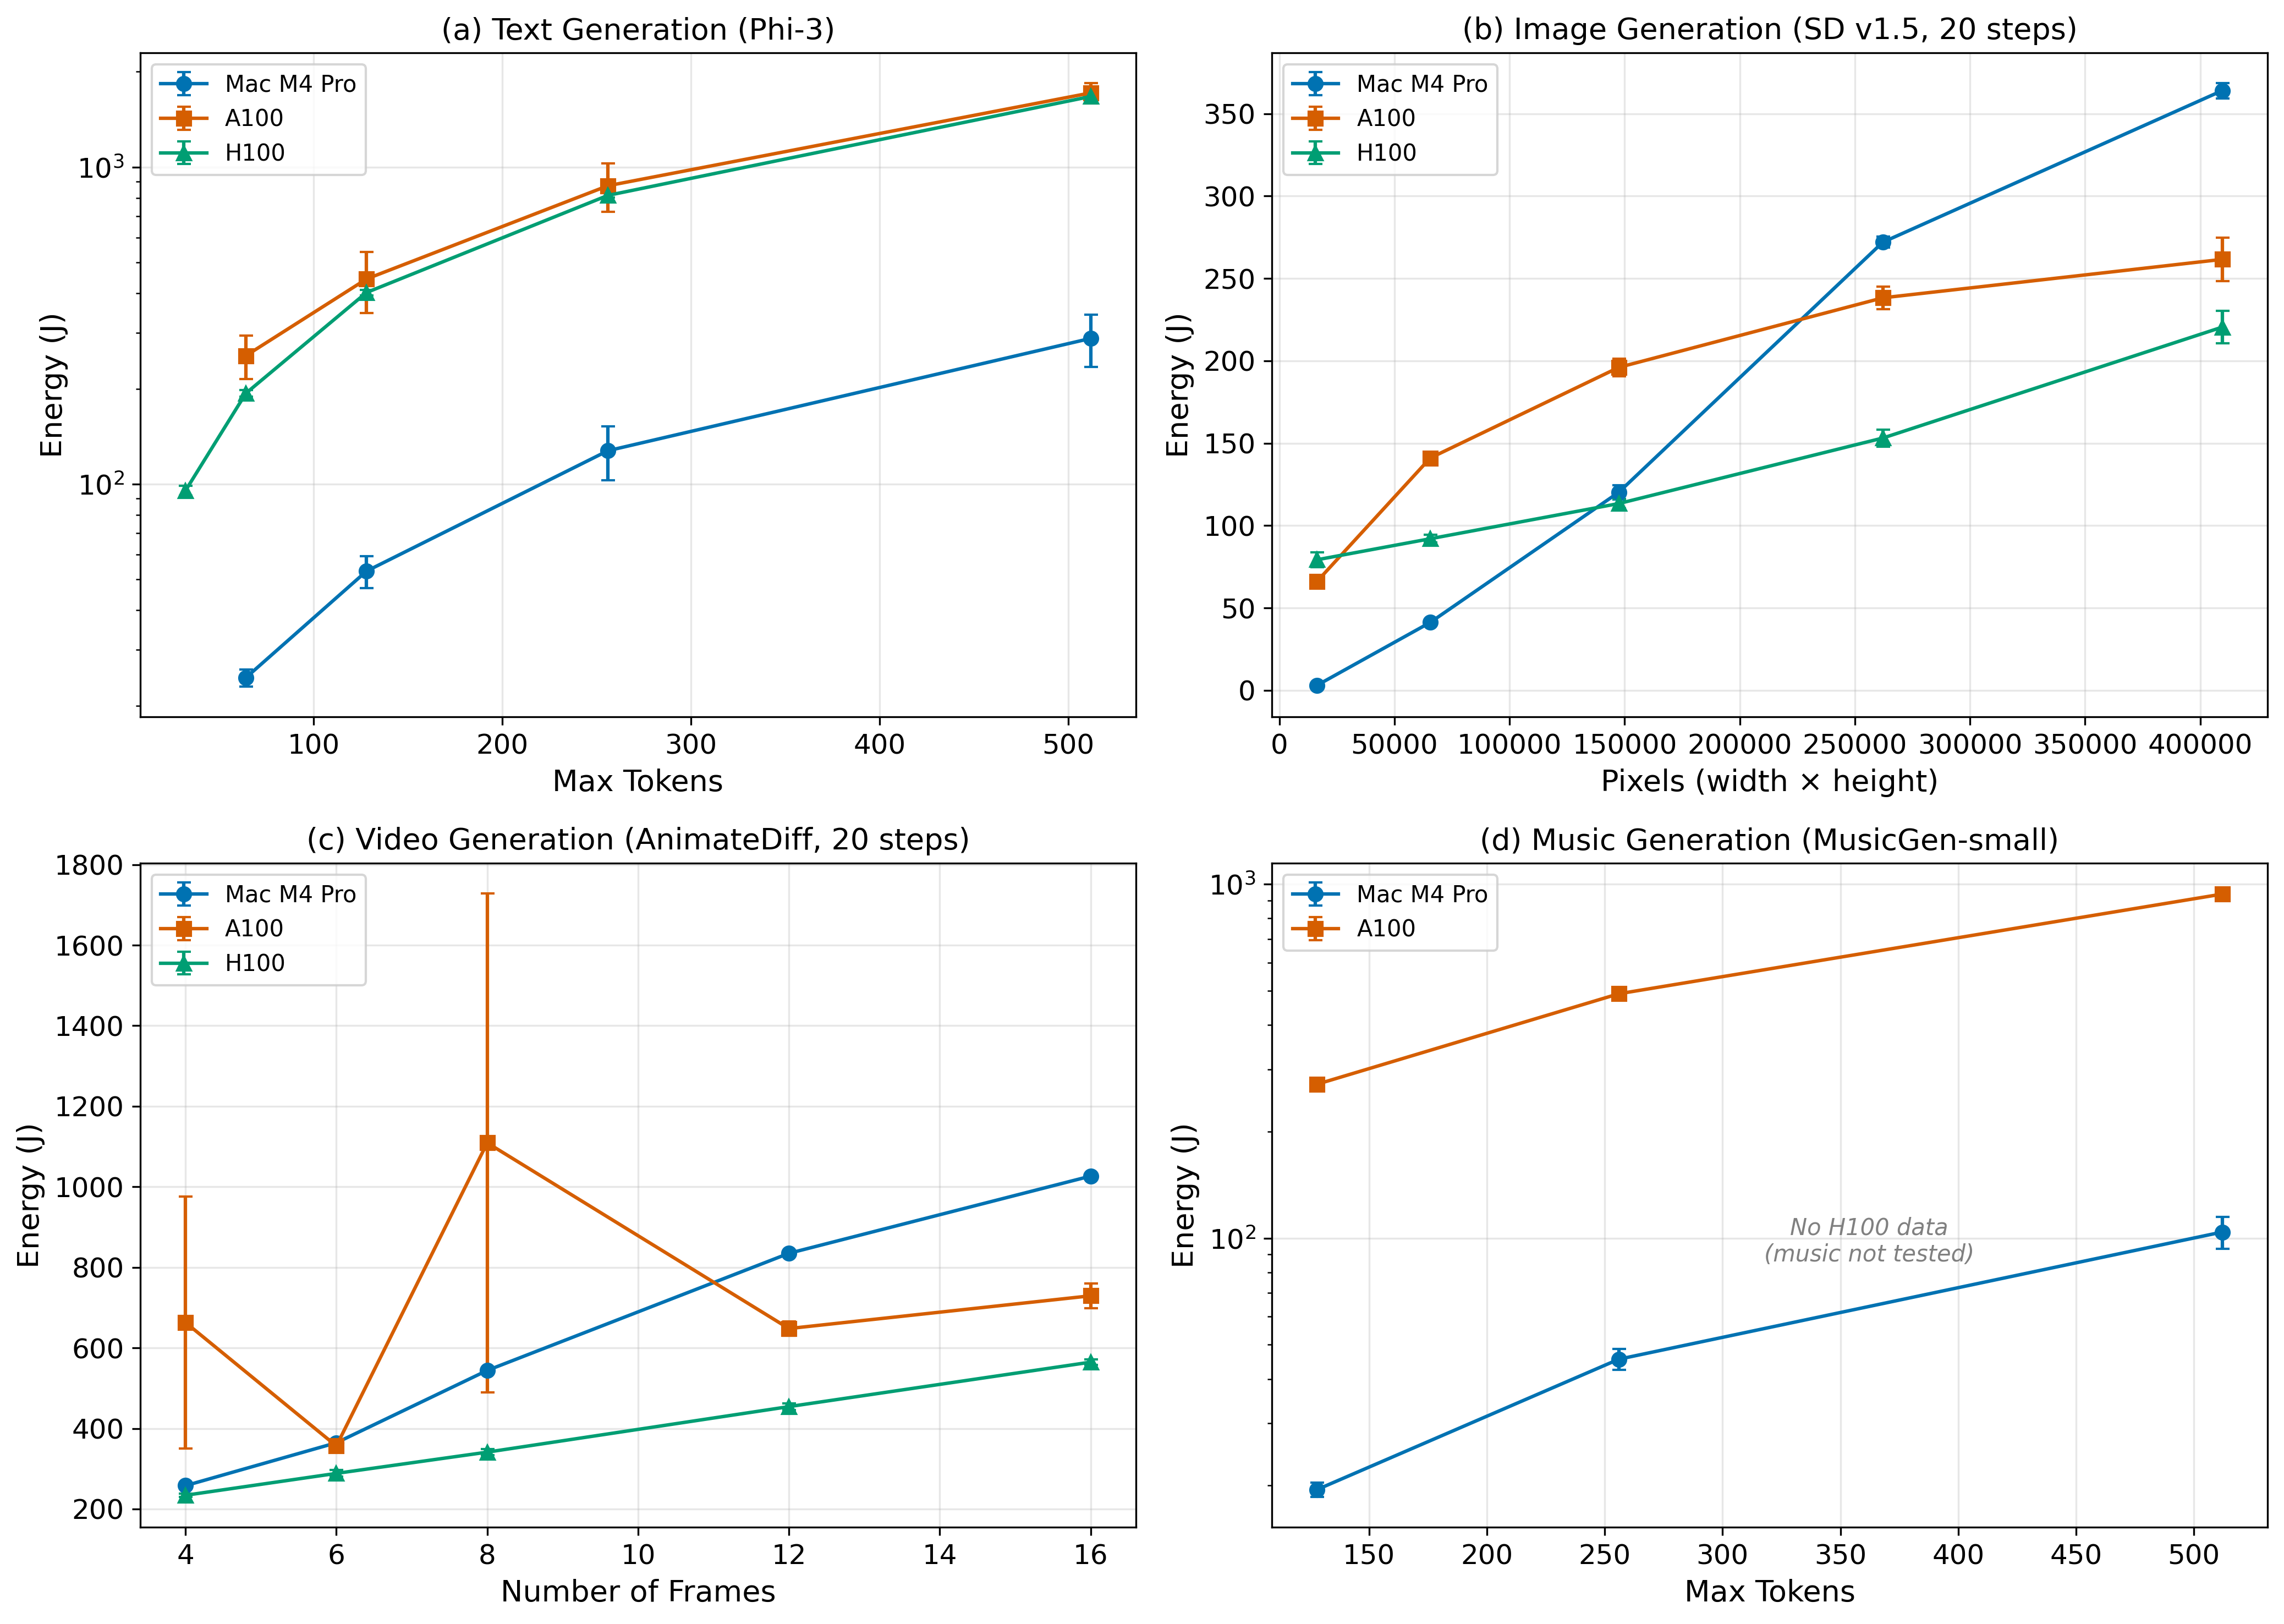
\includegraphics[width=0.95\textwidth]{figures/fig1_3hw_comparison.png}
\caption{\textbf{Energy consumption across four generative AI modalities on three hardware platforms.} Comparison of Apple M4 Pro (blue), NVIDIA A100 (vermillion), and NVIDIA H100 (teal) across (a)~text, (b)~image, (c)~video, and (d)~music generation. Error bars represent standard deviation over 30 runs. Dashed lines indicate crossover points. The H100 shifts crossover thresholds lower and eliminates the video crossover entirely.}
\label{fig:4modal}
\end{figure}

\subsection{Energy scaling laws reveal universal hardware divergence}

The H100's richer configuration space (5 resolutions $\times$ 6 step counts for SD~v1.5, 5 frame counts $\times$ 3 step counts for video) provides 5--6 data points per curve, improving fit confidence compared to the 3--4 points available for Mac and A100. Our fits should still be interpreted as \textit{empirical scaling relationships} ($R^2 > 0.97$ for most fits, with one exception: H100 image at $R^2 = 0.977$ when fit to 20-step data only) rather than as validated power laws. Table~\ref{tab:scaling} presents the fitted parameters.

Across all three platforms the same pattern holds: \textbf{the Mac exhibits superlinear scaling ($\beta > 1$)} while \textbf{GPUs show sublinear scaling ($\beta < 1$) for diffusion workloads}, producing the crossover points reported above. The one exception is H100 text generation ($\beta = 1.033$), which is near-linear---consistent with autoregressive workloads offering no parallelism advantage even on more powerful hardware. For diffusion modalities (image, video), both GPUs show clearly sublinear scaling, meaning their energy costs grow slower than workload complexity. The H100 shows slightly higher $\beta$ values than the A100 in diffusion modalities, reflecting its higher base power draw partially offsetting its greater compute throughput.

The divergence is most extreme for image generation ($\beta_\text{Mac} = 1.395$ vs $\beta_\text{A100} = 0.374$ vs $\beta_\text{H100} = 0.404$). The similar sublinear exponents for both GPUs, combined with the H100's lower effective intercept (due to faster completion at comparable power), explain the shifted crossover thresholds. For text and music, all platforms exhibit near-linear to superlinear scaling ($\beta \approx 0.96$--$1.20$), and the intercept difference ($\alpha_\text{GPU} / \alpha_\text{Mac} \approx 16$--$26\times$) precludes crossover within practical ranges.

Iyengar et al.~\cite{castano2025energy} previously reported power-law energy scaling for diffusion on GPUs. Our data add three observations: (1)~the exponent $\beta$ depends on hardware---sublinear on GPUs, superlinear on edge---while autoregressive workloads scale near-linearly everywhere; (2)~this platform-dependent exponent is what produces the crossover, which single-platform studies cannot detect; and (3)~newer GPU generations push the crossover lower, pointing toward broader GPU energy dominance for diffusion. We note that the image scaling law fits have lower $R^2$ for the H100 (0.977) than for text or video ($>$0.99), reflecting the two-dimensional nature of image complexity (resolution $\times$ steps) that a single-variable power law cannot fully capture. Detailed per-modality fits with residual analysis are provided in the Supplementary Information.

\begin{table}[t]
\centering
\caption{\textbf{Energy scaling law parameters} ($E = \alpha \cdot N^\beta$). Mac exhibits superlinear scaling ($\beta > 1$) across all modalities. GPUs show sublinear scaling ($\beta < 1$) for diffusion workloads (image, video) but near-linear scaling for autoregressive workloads (text). The exponent divergence is largest for image generation.}
\label{tab:scaling}
\small
\begin{tabular}{@{}llcccc@{}}
\toprule
\textbf{Modality} & \textbf{Scaling var.} & \textbf{Platform} & $\boldsymbol{\alpha}$ & $\boldsymbol{\beta}$ & $\boldsymbol{R^2}$ \\
\midrule
\multirow{3}{*}{Text} & \multirow{3}{*}{Tokens} & Mac M4 Pro & 0.167 & 1.195 & 0.9999 \\
 & & A100 & 4.330 & 0.959 & 0.9995 \\
 & & H100 & 2.660 & 1.033 & 0.9999 \\
\midrule
\multirow{3}{*}{Image} & \multirow{3}{*}{Pixels} & Mac M4 Pro & $8 \times 10^{-6}$ & 1.395 & 0.9998 \\
 & & A100 & 2.249 & 0.374 & 0.9974 \\
 & & H100 & 1.081 & 0.404 & 0.9770 \\
\midrule
\multirow{3}{*}{Video} & \multirow{3}{*}{Frames} & Mac M4 Pro & 59.20 & 1.065 & 1.0000 \\
 & & A100 & 155.19 & 0.570 & 0.9892 \\
 & & H100 & 88.18 & 0.665 & 0.9950 \\
\midrule
\multirow{2}{*}{Music} & \multirow{2}{*}{Tokens} & Mac M4 Pro & 0.058 & 1.200 & 1.0000 \\
 & & A100 & 3.205 & 0.910 & 0.9995 \\
\bottomrule
\end{tabular}
\end{table}

\subsection{Crossover points depend on both model architecture and GPU generation}

GPU generation shifts these crossover points substantially (Fig.~\ref{fig:ratio}):

\begin{itemize}[leftmargin=*]
\item \textbf{Image generation}: The Mac--A100 crossover occurs at $\sim$217,000 pixels ($\approx$466$\times$466), empirically confirmed between 384$^2$ and 512$^2$. The Mac--H100 crossover shifts to $\sim$142,000 pixels ($\approx$377$\times$377), empirically confirmed between 256$^2$ and 384$^2$---a 35\% reduction. This means the H100 is energy-competitive with the Mac across the entire standard Stable Diffusion resolution range (384$^2$ and above), whereas the A100 only wins at 512$^2$ and above.
\item \textbf{Video generation}: The Mac--A100 crossover occurs at $\sim$7 frames. For the H100, there is \textbf{no crossover}---it uses less energy than the Mac at \textit{all} tested sizes (4--16 frames, 9--46\% less). With H100-class hardware, video generation should always go to the GPU.
\item \textbf{Text and music}: No crossover on either GPU. The Mac remains 5.8--10.4$\times$ more efficient than both the A100 and H100 across all tested text configurations, and 9--14$\times$ more efficient for music.
\item \textbf{H100 vs A100}: The H100 is 35--45\% more energy-efficient than the A100 for image generation and 30--65\% for video, driven by 1.5--1.7$\times$ faster completion despite only modestly higher power draw ($\sim$1.3$\times$). For text, the H100 advantage is marginal (3--24\%).
\end{itemize}

In short, newer GPUs lower the crossover for diffusion workloads but barely help autoregressive ones. The architectural divide---serial versus parallel---appears to be a more durable determinant of optimal deployment than any single generation of hardware. If the trend continues (B100/B200), image crossover points will drop below 256$^2$, but text generation will likely remain edge-favoured until GPU idle power falls well below current levels or autoregressive decoding is replaced by a parallel alternative.

Practically, these crossover points can inform deployment policies. An AI serving platform with H100 GPUs should route all video requests and image requests at $\geq$384$^2$ to the GPU, while directing text and music queries to edge devices---or, if edge deployment is infeasible, maximising GPU batch utilisation. With A100-class hardware, the routing threshold shifts higher: only images at $\geq$512$^2$ and videos at $\geq$8 frames benefit from GPU routing.

\begin{figure}[t]
\centering
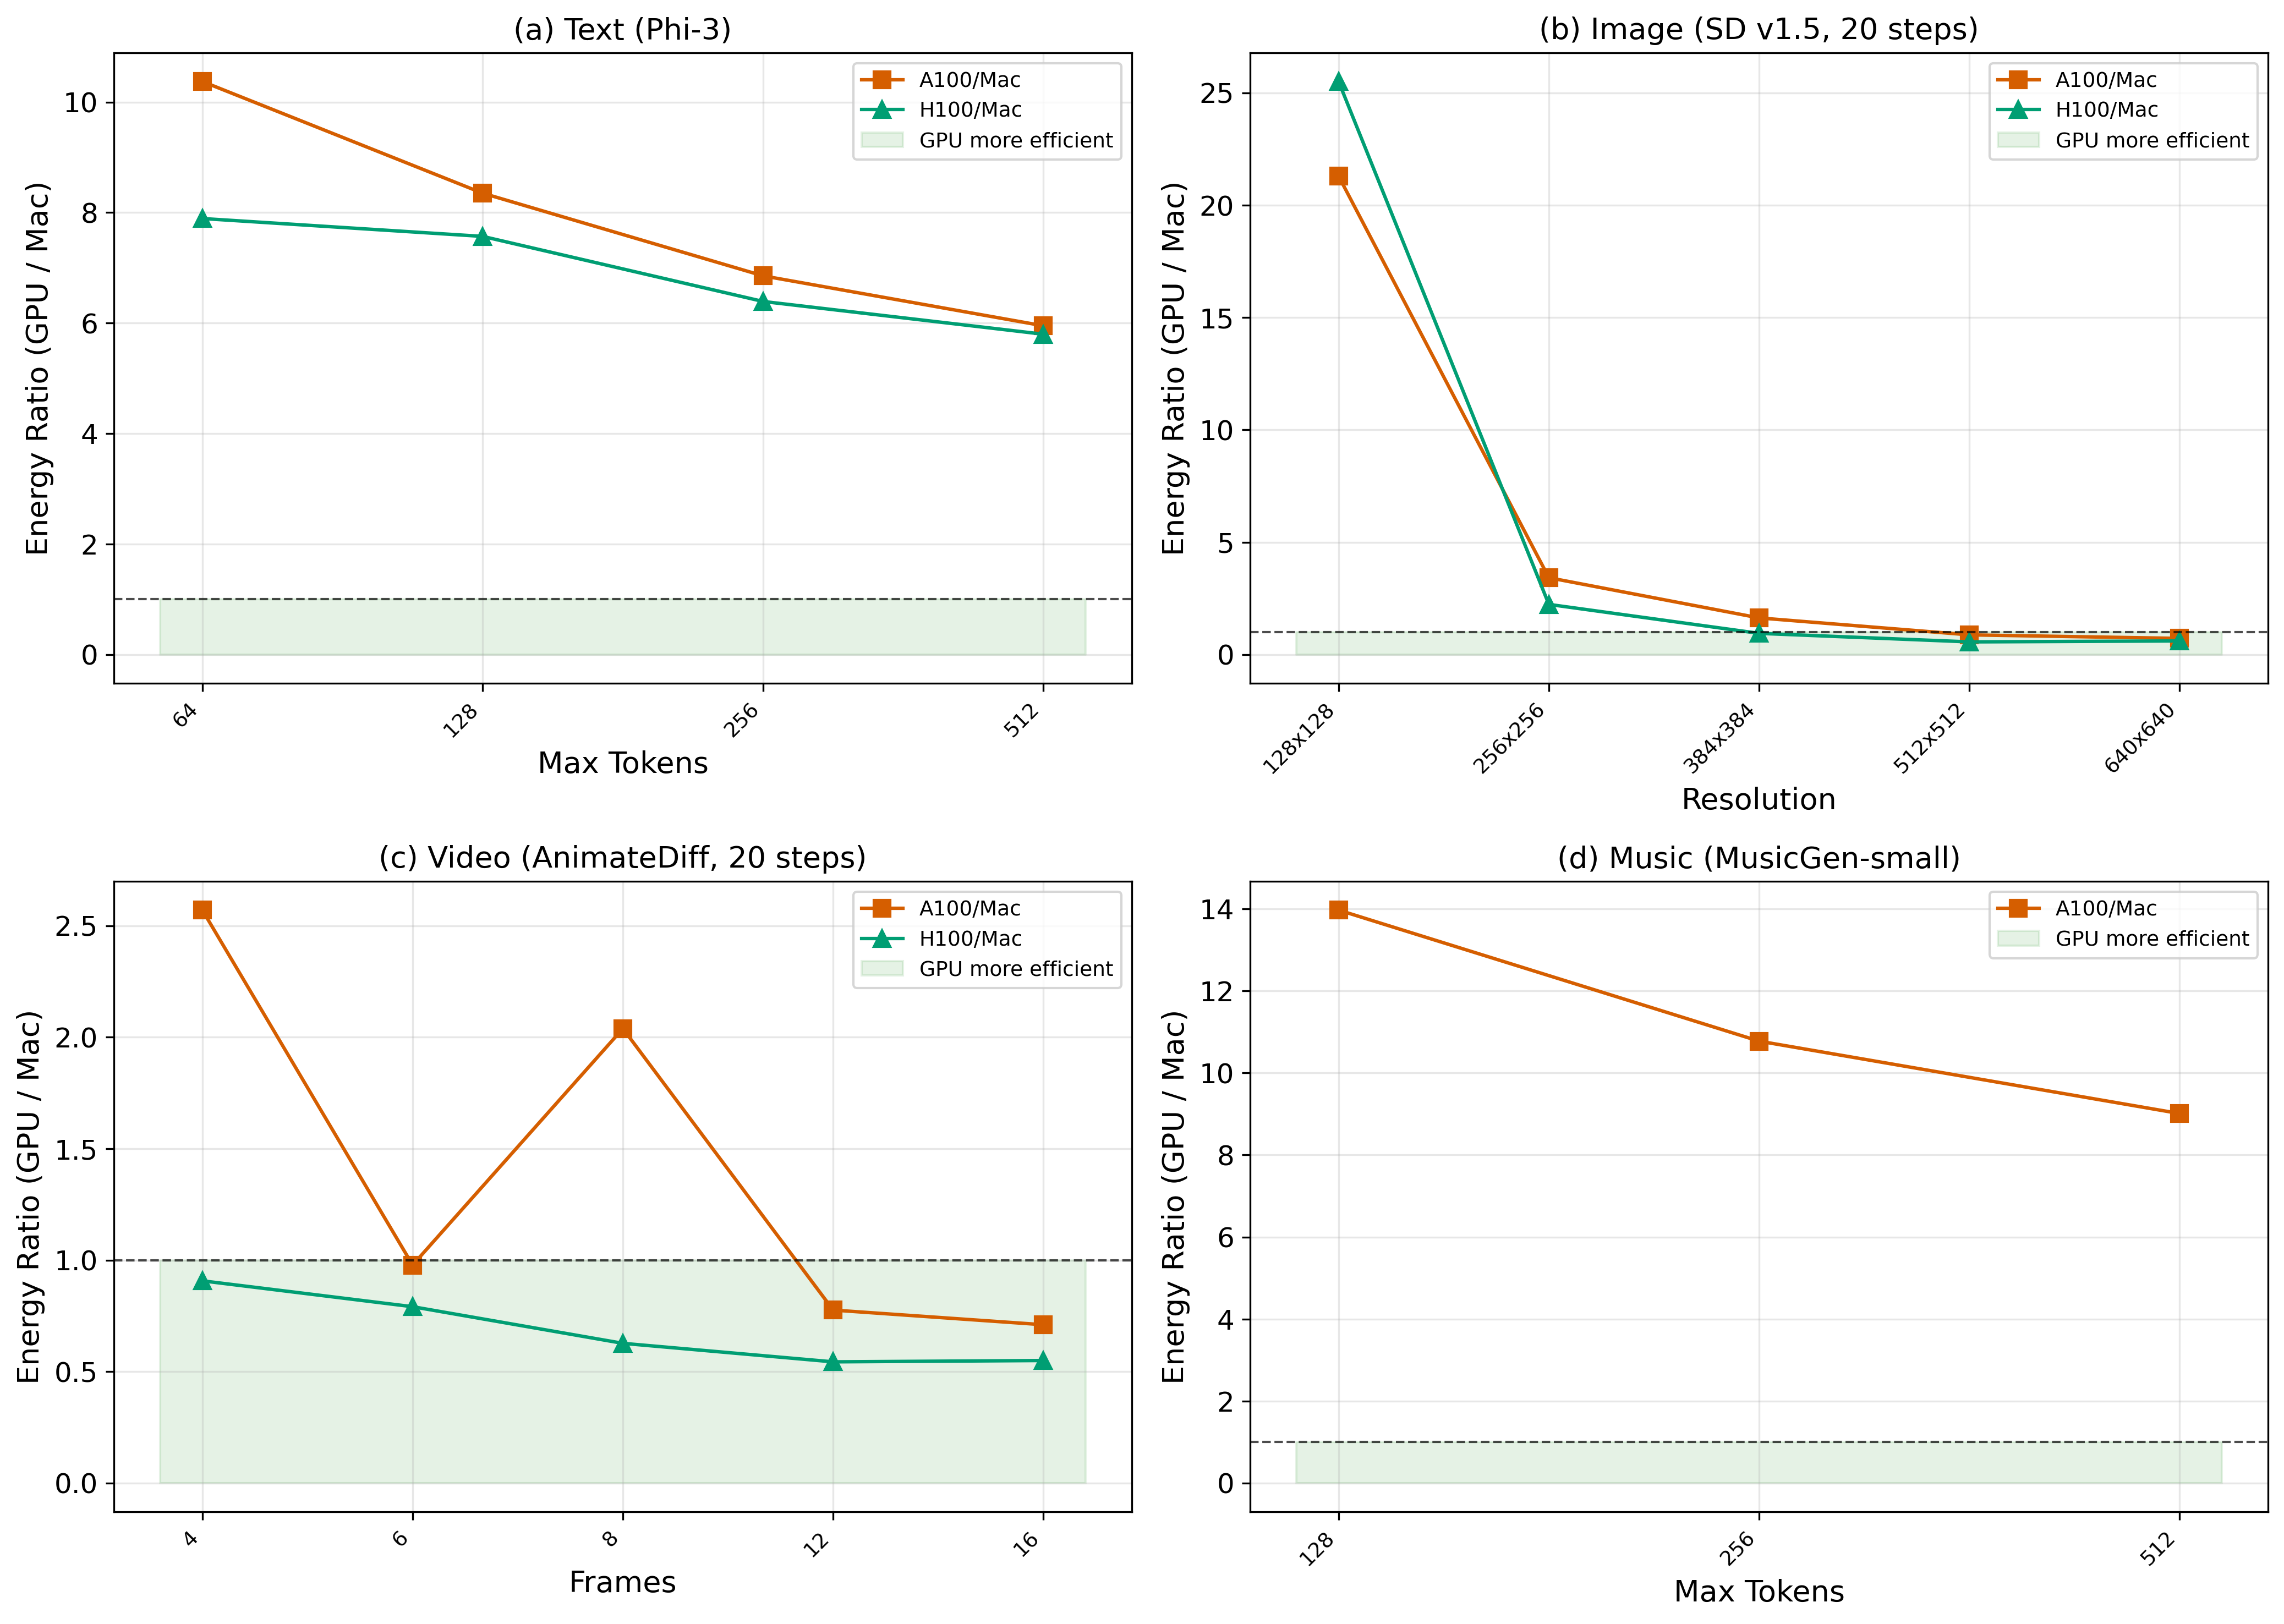
\includegraphics[width=0.95\textwidth]{figures/fig2_efficiency_ratio_3hw.png}
\caption{\textbf{Energy efficiency ratio across all configurations.} A100/Mac ratio (vermillion) and H100/Mac ratio (teal). Values below 1.0 indicate the GPU is more energy-efficient. The H100 crosses below 1.0 at lower complexity than the A100 for images, and remains below 1.0 for \textit{all} video configurations. Autoregressive modalities (text, music) consistently favour the Mac on both GPUs.}
\label{fig:ratio}
\end{figure}

\subsection{The speed--energy tradeoff reveals four regimes}

Figure~\ref{fig:tradeoff} maps each configuration in speed--energy space, where four operational regimes are visible:

\begin{enumerate}[leftmargin=*]
\item \textbf{Worst case} (slower, more energy): Music generation on GPUs---no speed gain, 9--14$\times$ energy penalty. The GPU's massive parallelism is entirely wasted on sequential token generation.
\item \textbf{Speed--energy tradeoff} (faster, more energy): Text generation and low-resolution image/video on A100---modest speedups insufficient to offset higher power draw.
\item \textbf{Best case} (faster, less energy): High-resolution image and multi-frame video on GPUs. The H100 extends this regime dramatically: it achieves the ``best case'' for \textit{all} video configurations and images at 384$^2$ and above, whereas the A100 only reaches this regime for images above 466$^2$ and videos above 7 frames.
\item \textbf{GPU generational leap}: The H100 occupies a distinct region from the A100, consistently shifted toward lower energy ratios. For video generation, the H100 moves entirely into the ``faster and cheaper'' quadrant, representing a qualitative improvement over the A100.
\end{enumerate}

\begin{figure}[t]
\centering
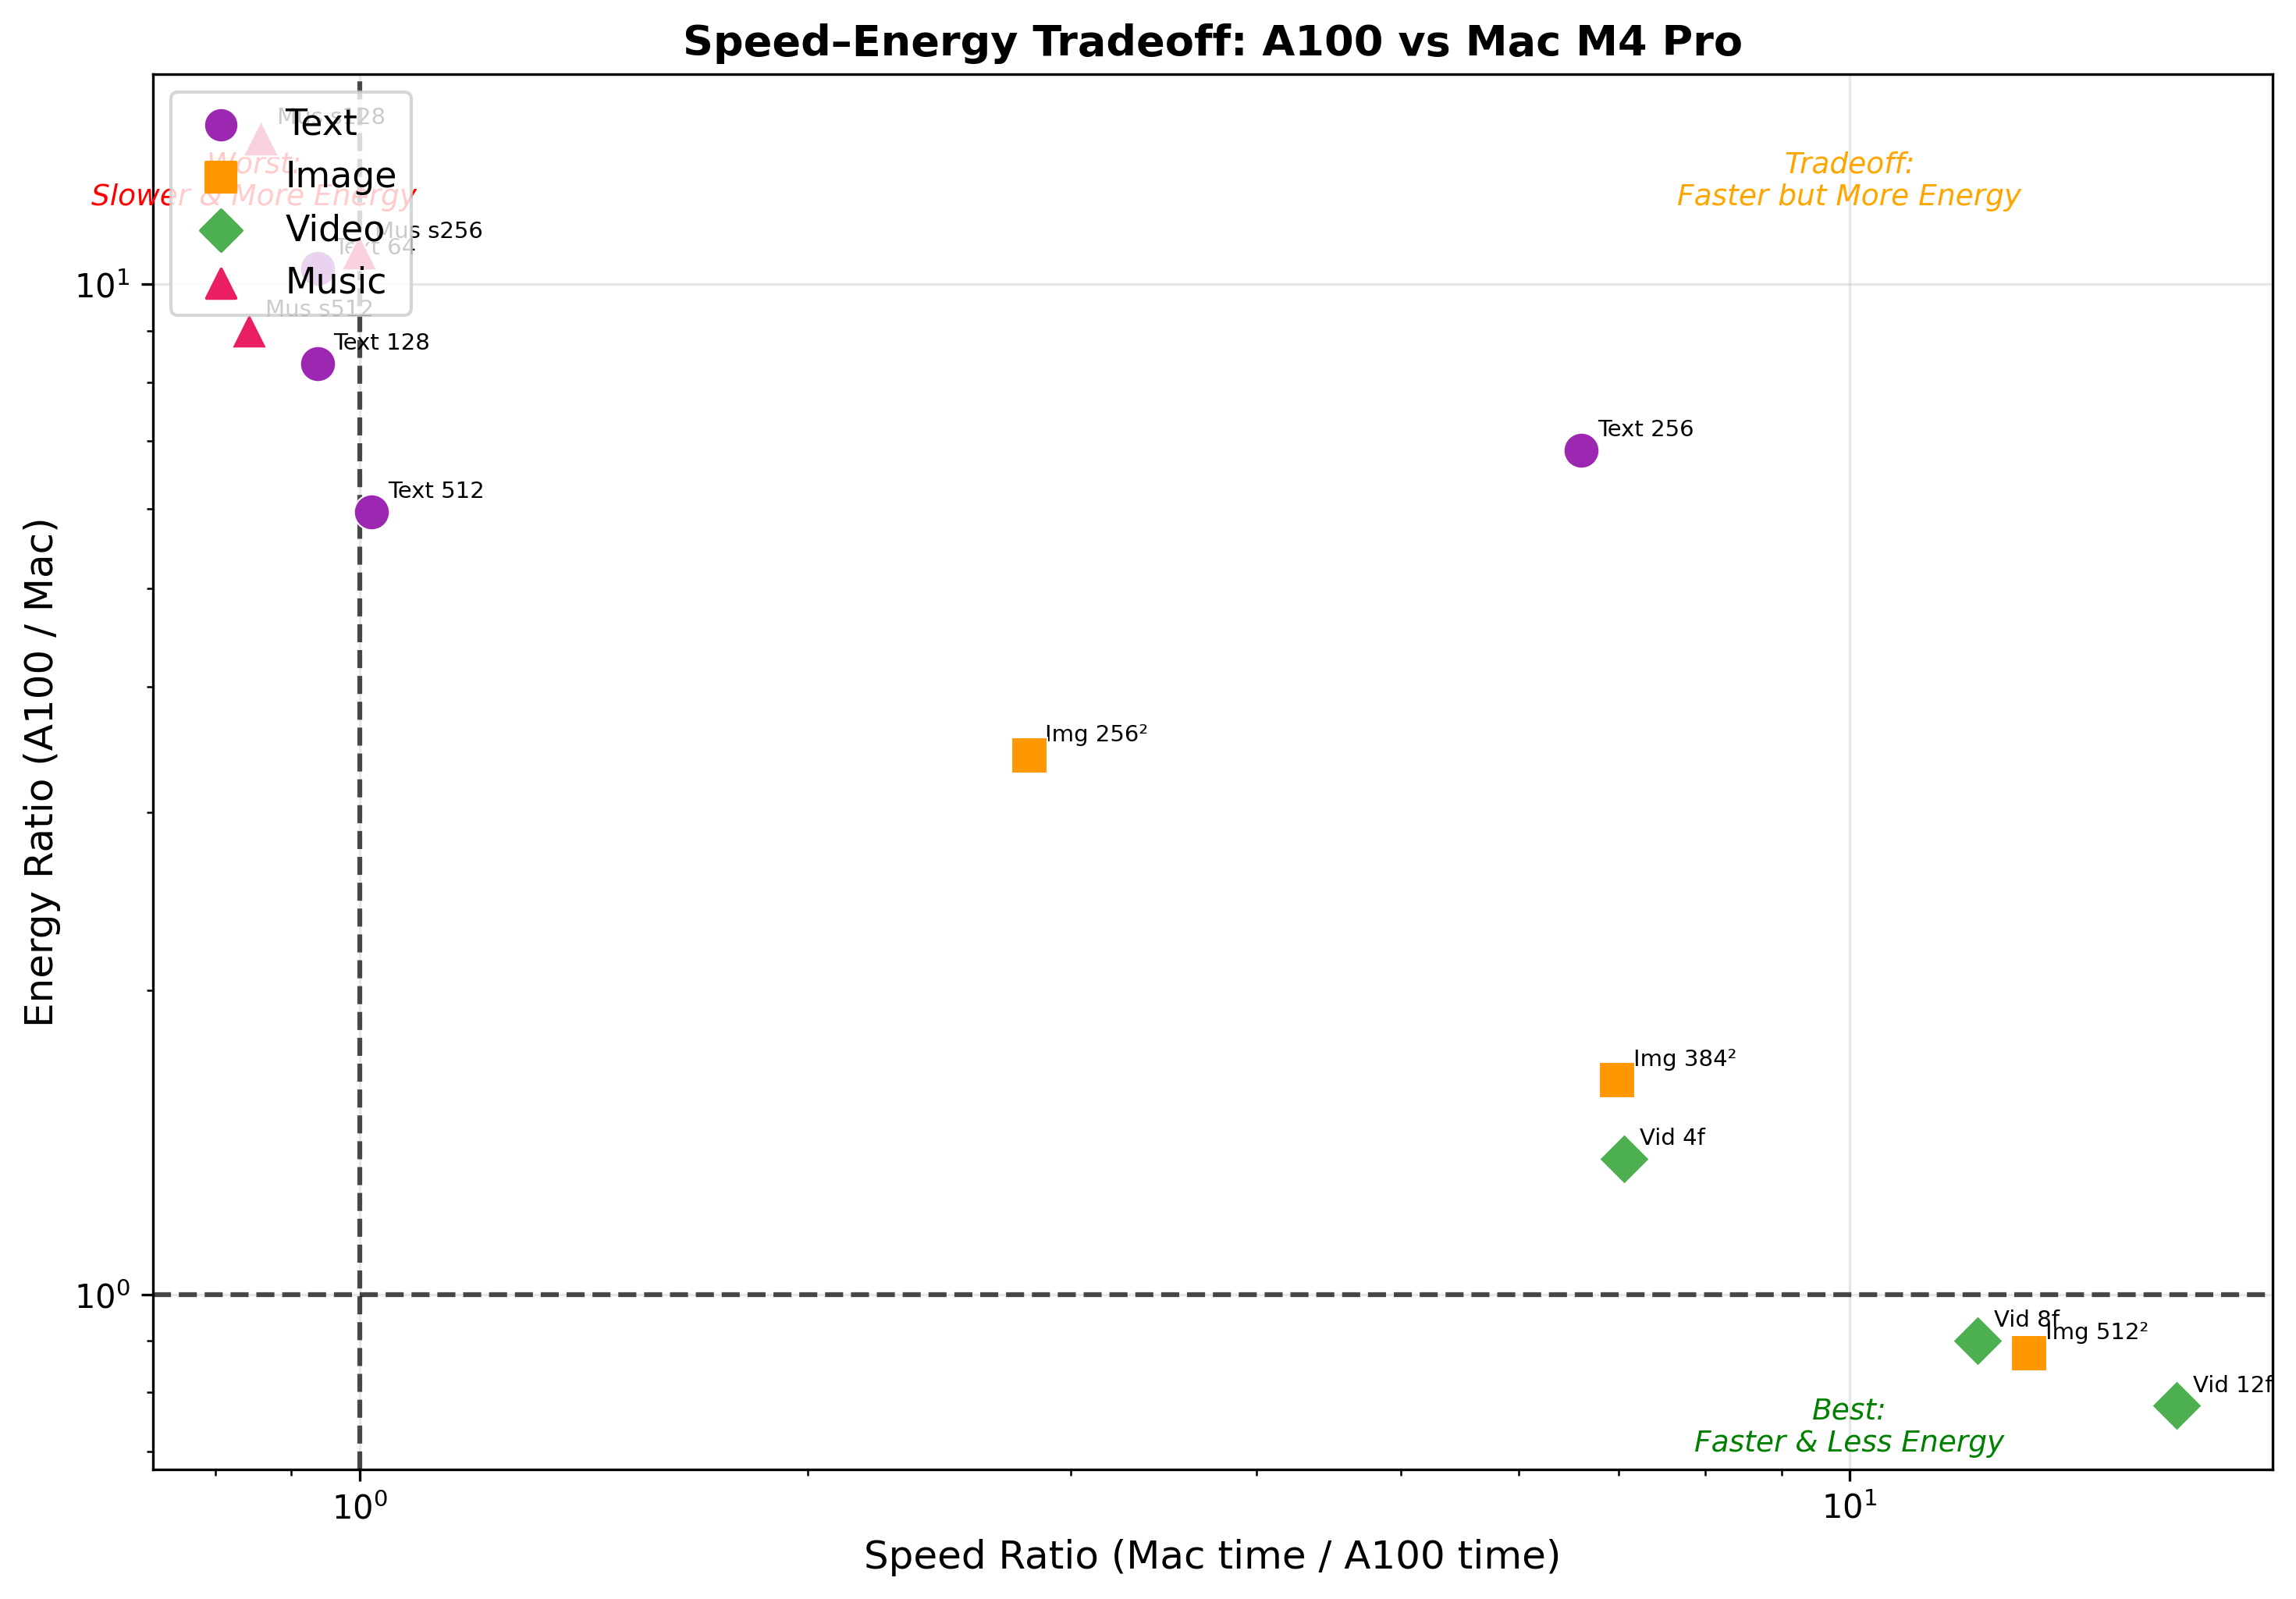
\includegraphics[width=0.85\textwidth]{figures/fig5_speed_energy_tradeoff.png}
\caption{\textbf{Speed--energy tradeoff across all configurations.} Each point represents a modality-configuration pair. Horizontal axis: speed ratio (Mac time / GPU time); vertical axis: energy ratio (GPU energy / Mac energy). A100 shown as circles, H100 as squares. Points below $y=1$ and right of $x=1$ represent the best case (faster and less energy on GPU). The H100 (teal) consistently sits lower than the A100 (vermillion) for diffusion workloads.}
\label{fig:tradeoff}
\end{figure}

\subsection{Power profiles explain the crossover mechanism}

Figure~\ref{fig:power} shows average and peak power across modalities. The A100 draws 63--279~W, the H100 125--412~W, and the Mac 6.4--24.3~W. What matters for energy is the ratio of speed gain to power increase: the H100 draws only $\sim$1.3$\times$ more than the A100 at matched configurations (e.g., 250~W vs 196~W for 384$^2$ images), but finishes 1.5--1.7$\times$ faster, netting 35--45\% energy savings.

For the crossover to occur, a GPU's speed advantage must exceed its power disadvantage: $\text{Speedup} > P_\text{GPU}/P_\text{Mac}$. Since $E = P \cdot t$, the GPU achieves lower energy when its time reduction factor exceeds its power increase factor:
\begin{itemize}[leftmargin=*]
\item H100 Image 384$^2$: speedup $\sim$22$\times$ $>$ power ratio $\sim$10$\times$ $\Rightarrow$ H100 wins
\item A100 Image 512$^2$: speedup 13.2$\times$ $>$ power ratio 5.9$\times$ $\Rightarrow$ A100 wins
\item H100 Video 4f: speedup $\sim$23$\times$ $>$ power ratio $\sim$12$\times$ $\Rightarrow$ H100 wins
\item Music: speedup 0.9$\times$ $<$ power ratio 9.9$\times$ $\Rightarrow$ Mac wins by $\sim$10$\times$
\end{itemize}

The H100's power depends heavily on utilisation: 160--190~W at 128$^2$ (23--27\% of its 700~W TDP), rising to 412~W at 640$^2$ (59\%). This 2.4$\times$ range mirrors the A100's pattern at a higher baseline. The Mac, by contrast, spans only $\sim$4$\times$ (6.4--24.3~W)---its SoC scales power smoothly but cannot exploit parallelism it does not have. Detailed per-configuration power measurements are provided in Supplementary Table~1.

\begin{figure}[t]
\centering
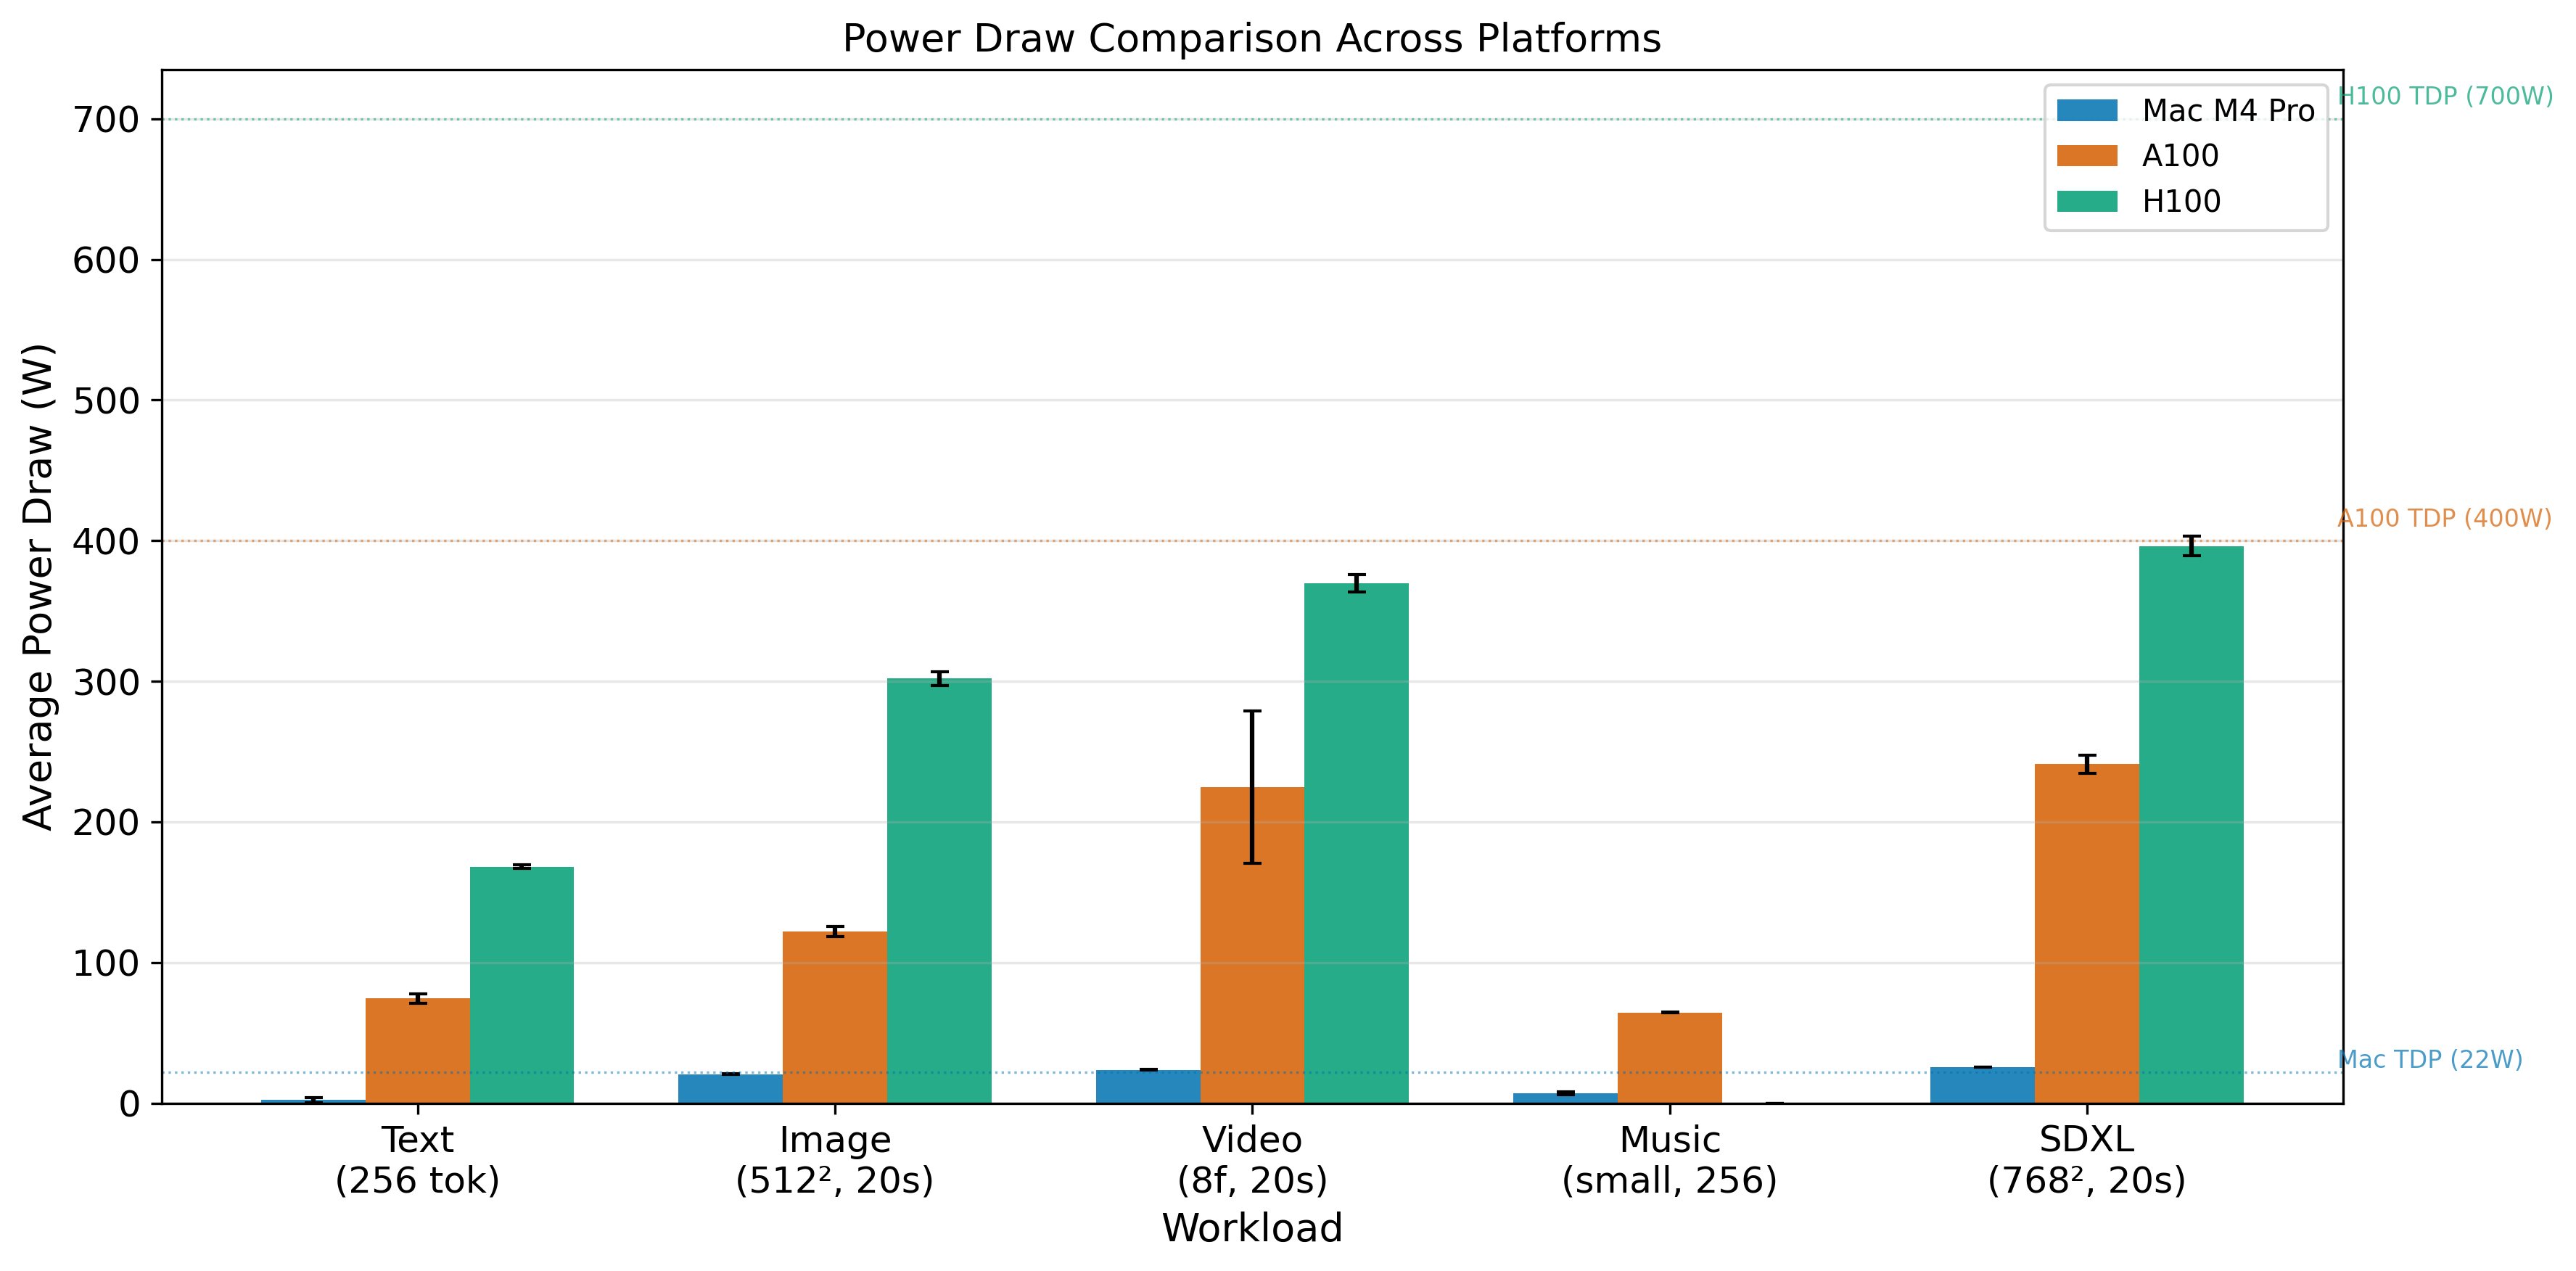
\includegraphics[width=0.95\textwidth]{figures/fig8_power_profile_3hw.png}
\caption{\textbf{Average and peak power draw across modalities on three platforms.} The H100 draws $\sim$1.3$\times$ more power than the A100 but achieves 1.5--1.7$\times$ faster completion, explaining its superior energy efficiency for diffusion workloads. The Mac's power varies by only $\sim$4$\times$ across workloads, reflecting uniform utilization.}
\label{fig:power}
\end{figure}

\subsection{Cross-model validation: SDXL confirms architecture-driven patterns}

To validate that our findings generalise beyond a single model per modality, we repeated the image generation experiments with SDXL-base-1.0~\cite{podell2023sdxl} (3.5B parameters, 3.9$\times$ larger than SD~v1.5) across all three platforms. The crossover pattern persisted with two notable features. First, the H100 consumed 35--40\% less energy than the A100 at matched configurations, consistent with the SD~v1.5 pattern. Second, the H100 achieved energy parity with the Mac at lower resolutions than for SD~v1.5, consistent with SDXL's higher computational intensity providing better GPU utilisation---the larger UNet generates more FLOPs per denoising step, pushing GPU utilisation above the crossover threshold at smaller spatial dimensions.

On the H100, SDXL at 1024$^2$/30 steps consumed 945~J with a CLIP score of 0.33, while SD~v1.5 at 640$^2$/50 steps consumed 537~J with CLIP~0.29---demonstrating that SDXL delivers meaningfully higher quality at a proportional energy cost. This result has practical significance: practitioners choosing between models face an energy--quality tradeoff that depends on hardware. On the Mac, the energy penalty for switching from SD~v1.5 to SDXL is disproportionately large due to the Mac's superlinear scaling, whereas on GPUs the penalty is modest relative to the quality gain.

\subsection{Batched inference narrows but does not eliminate the edge advantage}
\label{sec:batched}

Real-world GPU serving systems batch multiple queries to amortize fixed power costs. We measured batched Phi-3 inference on both the A100 and H100 with batch sizes 1--16. Per-query energy dropped dramatically: on the H100, from 889~J (batch=1) to 69~J (batch=16), a 92\% reduction; on the A100, from 876~J to 115~J, an 87\% reduction. The energy--batch relationship follows a near-inverse pattern: doubling the batch size approximately halves per-query energy, consistent with amortisation of fixed power costs (idle GPU power, memory controller overhead) across queries.

However, even at batch=16, the H100's per-query energy (69~J) remains 2.8$\times$ higher than the Mac's single-query energy (24.5~J at 64 tokens). Extrapolating the batching trend, the H100 would require batch sizes of $\sim$45 to match the Mac's per-query energy---a utilisation level rarely sustained in practice outside the largest serving deployments. This confirms that batching substantially improves GPU efficiency but does not overturn the edge advantage for autoregressive workloads at the model sizes tested. For larger models (70B+) that exceed edge memory capacity, GPU batching remains the only viable option, and the 92\% per-query reduction at batch=16 underscores the importance of maximising GPU utilisation in such deployments.

\subsection{Energy--quality tradeoff: CLIP scores reveal diminishing returns}

We measured CLIP scores (image--text alignment) alongside energy for SD~v1.5 and SDXL across all three platforms with identical prompts and seeds. Three patterns emerged. First, quality saturated well before maximum step counts: on the H100, SD~v1.5 reached CLIP $\approx$0.30 at 512$^2$ by 15 steps, while additional steps to 50 consumed 2.4$\times$ more energy with no quality improvement. SDXL showed a similar pattern with saturation at $\sim$15 steps (CLIP $\approx$0.33 at 1024$^2$). Second, resolution had a larger effect on quality than step count: increasing from 256$^2$ to 512$^2$ improved CLIP by 0.08--0.10 points, while increasing steps from 20 to 50 at fixed resolution improved CLIP by only 0.01--0.02.

Third, and most practically relevant, the energy--quality Pareto frontier is hardware-dependent. On the Mac, the most energy-efficient path to high quality is moderate resolution with minimal steps (384$^2$/15 steps: CLIP 0.28, 16~J). On the H100, higher resolution becomes energy-competitive (512$^2$/15 steps: CLIP 0.30, 140~J), and the marginal energy cost per CLIP-point improvement is substantially lower than on the Mac at high resolutions. These findings suggest that energy-quality-aware scheduling---routing to the optimal hardware \textit{and} truncating denoising at the quality saturation point---could reduce consumption by 50--60\% at negligible quality cost. Full CLIP score data across all configurations and platforms are provided in the Supplementary Information (Supplementary Fig.~7).

%% ============================================================
\section{Discussion}
\label{sec:discussion}
%% ============================================================

The three-platform comparison points to a concrete opportunity: a \textit{modality-aware, hardware-aware routing strategy} that directs each query to the cheapest hardware for its workload type, with thresholds that depend on the available GPU generation. Text generation (LLM inference) dominates current AI workloads, with an estimated 13 billion daily queries~\cite{devries2023growing}. Routing these autoregressive workloads to edge devices would reduce per-query energy by 6--10$\times$, regardless of whether the alternative is an A100 or H100.

For diffusion workloads, the optimal routing depends on the available GPU: with H100-class hardware, \textit{all} video and standard-resolution image generation ($\geq$384$^2$) should be GPU-routed for energy savings of 6--46\%. With A100-class hardware, only high-resolution images ($\geq$512$^2$) and longer videos ($\geq$8 frames) benefit from GPU routing. This hardware-dependent policy has practical implications: organisations with newer GPU fleets can route more aggressively to GPUs, while those with older hardware should retain more workloads on edge.

As an illustrative upper bound, we project that if all single-query autoregressive inference (text, music) were routed from GPU to edge, and diffusion workloads were routed to the most efficient available GPU, the energy reduction would be approximately 200--400~GWh annually, accounting for batching (3--8$\times$ GPU efficiency improvement~\cite{wu2022sustainable}), partial edge coverage, and the fact that many production queries target models too large for current edge hardware (70B+). While uncertain, even conservative estimates suggest substantial savings from modality-aware routing.

This fits naturally into the broader trend toward hybrid AI architectures, where lightweight models run on-device for latency and privacy while complex tasks go to cloud GPUs~\cite{xu2024edge}. Energy efficiency adds a \textit{third} reason for this split, and unlike latency or privacy, the optimal split point can be read off a scaling curve. No model modification is needed: the same Phi-3 checkpoint runs on both platforms, and the routing decision depends only on the modality and input complexity.

Implementation is straightforward: an inference scheduler classifies each request by modality and complexity (resolution, frame count, or token length) and routes it to the platform whose energy profile is favourable for that configuration. Our crossover thresholds provide the decision boundaries. For organisations operating mixed fleets (e.g., edge devices for local inference and cloud GPUs for burst capacity), this approach can reduce energy consumption without sacrificing throughput or quality. The batching results further inform scheduling: when GPU utilisation is high (batch $\geq$8), the per-query energy gap narrows substantially, making GPU routing more competitive even for text---though edge deployment remains preferable at low utilisation.

The crossover effect arises from a fundamental mismatch between computational paradigm and hardware design. Autoregressive models generate tokens sequentially, creating an inherently serial computation graph. The A100's 6,912 CUDA cores operate at high base power (63--80~W even for small workloads) but cannot accelerate sequential generation proportionally. The Mac's unified memory architecture eliminates data transfer overhead and operates at 6--12~W total system power, making it 9--14$\times$ more energy-efficient. Diffusion models~\cite{ho2020denoising}, by contrast, perform parallel denoising across spatial dimensions~\cite{rombach2022high,guo2024animatediff}, creating workloads that can saturate GPU cores. At low resolutions the workload is insufficient to justify the GPU's power overhead, but as resolution increases, GPU utilization improves dramatically: the A100 completes 512$\times$512 generation 13$\times$ faster than the Mac, and this speedup exceeds the 6$\times$ power penalty. This mechanism is reflected in our scaling fits: the Mac's superlinear exponent ($\beta > 1$) is consistent with memory bandwidth saturation at higher complexity, while the GPUs' sublinear exponents ($\beta < 1$) for diffusion workloads reflect improving utilization. The H100's text exponent ($\beta = 1.033$, near-linear) reinforces the point: longer sequences do not create more parallelism for autoregressive decoding. The H100's advantage over the A100 for diffusion is instructive: despite $\sim$1.3$\times$ higher power, it completes tasks 1.5--1.7$\times$ faster, yielding 35--45\% energy savings. This disproportionate speedup arises because the H100's 2.4$\times$ more CUDA cores and 1.7$\times$ higher memory bandwidth improve throughput faster than they increase power draw. For autoregressive workloads, neither additional cores nor bandwidth helps, and the H100 is only marginally better (3--24\%) than the A100. We note an alternative explanation: constant idle power captured by \texttt{powermetrics} (Mac) but excluded from \texttt{pynvml} (GPUs) could inflate the Mac's superlinearity. Our sensitivity analysis (below) suggests this does not change qualitative conclusions, but dedicated system-level measurement would resolve this definitively.

Our findings extend and contextualise several prior results. Luccioni et al.~\cite{luccioni2024power} found that image generation uses $\sim$60$\times$ more energy than text classification on an A100; we show that this gap is hardware-dependent, with text and music becoming disproportionately cheaper on edge hardware. GPU-only benchmarks~\cite{you2023zeus} may overestimate autoregressive inference costs by an order of magnitude relative to edge deployment. Samsi et al.~\cite{samsi2023words} found approximately linear energy-per-token scaling, consistent with our fits ($\beta \approx 0.96$--$1.20$). Iyengar et al.~\cite{castano2025energy} found FLOPs-based power-law scaling for diffusion on GPUs; we complement this by showing qualitatively different scaling on edge SoCs.

Comparing the A100 and H100 generations suggests a trend: each new GPU generation lowers the crossover for diffusion workloads while leaving the autoregressive gap largely unchanged. The A100-to-H100 transition reduced the image crossover from $\sim$466$^2$ to $\sim$377$^2$ (35\% reduction) and eliminated the video crossover entirely. If this trend continues (B100/B200), we predict the image crossover will drop below 256$^2$, making GPUs energy-dominant across all practical resolutions; music may eventually cross over as GPU idle power decreases; but text generation will remain edge-favoured until GPU idle power drops below $\sim$30~W or autoregressive architectures are replaced by parallel alternatives. The emergence of dedicated AI accelerators (Google TPU v5, AMD MI300X) may further diversify the landscape; our framework of measuring energy scaling exponents and fitting crossover points provides a general methodology applicable to any hardware pairing.

There is also a methodological point. Existing AI energy benchmarks~\cite{you2023zeus,jegham2025hungry,luccioni2024power} report values on fixed hardware, implicitly treating deployment as a constant. Our data show that this can mislead: a model that looks energy-hungry on a GPU may be cheap on edge hardware, and vice versa. Future benchmarks should cover at least two hardware tiers, and efficiency claims should state the deployment context.

The Pareto analysis of energy versus quality further enriches the deployment picture. Our CLIP measurements show that quality saturates well before maximum denoising steps, meaning that a quality-aware scheduler could truncate generation at the saturation point and redirect saved energy to additional queries. Combined with hardware-aware routing, this yields a two-dimensional optimization: choose the right hardware for the modality, then choose the right quality operating point for the application. For applications tolerant of lower quality (thumbnails, previews), the Mac at moderate resolution provides an extremely energy-efficient option; for production-quality content, the H100 at optimal step count represents the best energy-quality tradeoff.

\subsection{Limitations}

Several limitations deserve mention. First, GPU measurements via \texttt{pynvml} capture GPU board power only, excluding CPU and system overhead. Mac measurements via \texttt{powermetrics} include all subsystems. This asymmetry may slightly underestimate GPU total energy; however, for inference workloads, GPU power dominates total system consumption~\cite{patterson2021carbon,wu2022sustainable}. To assess sensitivity, we applied a conservative 40\% overhead correction to all GPU measurements (the upper bound estimated by Wu et al.~\cite{wu2022sustainable} for host system contribution). Even with this correction, the autoregressive advantage remains 4.1--7.4$\times$ (vs.\ 5.8--14$\times$ uncorrected), the crossover effect persists, and all qualitative conclusions hold.

Second, all tested models are in the 589M--3.8B parameter range. We deliberately chose edge-deployable models because the crossover question is only meaningful when both deployment options are viable: a 70B-parameter model~\cite{touvron2023llama} cannot run on a 24~GB edge device, so no crossover decision exists. However, this scope limits direct applicability to the growing class of production models (GPT-4, LLaMA-3-70B) that require GPU deployment. For these larger models, our batching results (Section~\ref{sec:batched}) provide the relevant insight: maximising GPU utilisation through batching reduces per-query energy by up to 92\%, which becomes the primary efficiency lever when edge deployment is infeasible. As edge hardware memory grows (Apple M4 Ultra: 192~GB, Qualcomm Snapdragon X: 64~GB), the crossover analysis will become relevant for increasingly large models. We also note that model distillation and quantization (4-bit GPTQ, AWQ) are rapidly expanding the range of models deployable on edge; our framework can be directly applied to evaluate the energy tradeoffs of quantized variants.

Third, our Colab-based GPU measurements may be affected by multi-tenant variability. However, our 30-repeat protocol yielded low coefficients of variation (0.6--2.9\% for image/video; Table~\ref{tab:reliability}), suggesting stable GPU allocation. We confirmed consistent GPU clock speeds and memory utilization across runs.

Fourth, we incorporate CLIP scores for image quality assessment on all three platforms, enabling preliminary energy--quality Pareto analysis. However, more comprehensive quality evaluation (FID, FVD, perplexity, CLAP) across all modalities would strengthen the energy--quality tradeoff analysis.

Fifth, while the H100's denser configuration space provides more data points per curve, the scaling law fits for image generation show lower $R^2$ (0.977) than for text or video, reflecting the two-dimensional nature (resolution $\times$ steps) of image complexity that a single-variable power law cannot fully capture. Future work should explore multi-variable scaling models.

Sixth, the platforms use different PyTorch versions (2.4.1 on Mac, 2.10.0 on GPUs due to Colab constraints), which may introduce software-level performance differences. Seventh, we validate prompt invariance by testing 5 diverse prompts per modality (text and image) on Mac M4 Pro and confirm that the between-prompt variance is 13--14$\times$ smaller than within-prompt run-to-run variance (Supplementary Note~5, Supplementary Fig.~10). Image generation shows only 2.0\% maximum range across prompts; text shows 11.0\% (driven by input length differences), confirming that computational configuration, not prompt content, determines energy consumption. Eighth, we do not account for network transfer energy in cloud deployment or model quantization effects. Finally, testing consumer GPUs (RTX 4090), mobile SoCs (Qualcomm Snapdragon X Elite), and DiT-based image models would further strengthen generalizability.

\begin{table}[t]
\centering
\caption{\textbf{Measurement reliability.} Coefficient of variation (CV) across 30 runs for representative configurations. Image and video measurements show excellent reproducibility ($<$3\%). Text CV is higher (17--19\%) due to variable output lengths from early EOS tokens. Music uses stochastic sampling (top-$k$=250), introducing additional variance.}
\label{tab:reliability}
\small
\begin{tabular}{@{}llccc@{}}
\toprule
\textbf{Modality} & \textbf{Configuration} & \textbf{Mac CV (\%)} & \textbf{A100 CV (\%)} & \textbf{H100 CV (\%)} \\
\midrule
Text & 256 tokens & 19.5 & 17.7 & 1.6 \\
Image & 512$\times$512, 20 steps & 1.3 & 2.9 & 3.4 \\
Video & 8 frames, 20 steps & 0.6 & 2.7 & 2.2 \\
Music & Small, 256 tokens & 6.9 & 0.6 & -- \\
\bottomrule
\end{tabular}
\end{table}

%% ============================================================
\section{Conclusion}
\label{sec:conclusion}
%% ============================================================

This study presents the first cross-hardware, cross-modality energy benchmark for generative AI inference, spanning three hardware tiers (edge SoC, mainstream GPU, high-end GPU), 4,500 runs, 6 models, and 76 configurations. Our key findings are as follows.

First, we identify and quantify the \textbf{Energy Crossover Effect}: for diffusion-based workloads (image and video generation), energy-efficiency leadership shifts from edge hardware to GPUs as output complexity grows. Autoregressive workloads (text and music) consistently favour edge hardware by 6--14$\times$, regardless of complexity or GPU generation.

Second, we establish \textbf{modality-specific energy scaling laws} ($E = \alpha \cdot N^\beta$), revealing that the edge platform exhibits superlinear scaling ($\beta > 1$) while GPUs exhibit sublinear scaling ($\beta < 1$) for diffusion workloads. This divergence in scaling exponents produces predictable crossover points that are absent in autoregressive tasks.

Third, we demonstrate that \textbf{GPU generation shifts the crossover threshold}: the H100 reaches energy parity with the Mac between 256$^2$ and 384$^2$ pixels for image generation (vs.\ $\sim$466$^2$ for A100) and eliminates the video crossover entirely, being more energy-efficient at all tested frame counts. This trend suggests that future GPU generations will make GPUs energy-dominant across all practical diffusion workloads.

Fourth, these measurements yield actionable \textbf{deployment guidelines}: an inference scheduler that routes requests based on modality and complexity---directing autoregressive workloads to edge devices and diffusion workloads above the crossover threshold to GPUs---can reduce per-query energy consumption by up to an order of magnitude. We estimate annual energy savings of 200--400~GWh under optimistic deployment assumptions.

Future work should extend this framework to larger models, additional hardware platforms (consumer GPUs, TPUs, mobile SoCs), and emerging architectures such as Diffusion Transformers (DiT). Incorporating network transfer energy, multi-variable scaling models, and comprehensive quality metrics across all modalities would further refine the energy-aware routing strategies proposed here.

%% ============================================================
%% CRediT author statement
%% ============================================================

\section*{CRediT authorship contribution statement}

\textbf{Yongjun Kim:} Conceptualization, Methodology, Software, Formal analysis, Investigation, Data curation, Writing -- original draft, Visualization. \textbf{Seoksoo Kim:} Supervision, Validation, Writing -- review \& editing.

%% ============================================================
%% Data Availability
%% ============================================================

\section*{Data availability}

All experimental data (4,500 JSON records across three hardware platforms), analysis scripts, and measurement notebooks are available at \url{https://github.com/yjkim0123/energy-crossover-effect}.

%% ============================================================
%% Declaration of competing interest
%% ============================================================

\section*{Declaration of competing interest}

The authors declare that they have no known competing financial interests or personal relationships that could have appeared to influence the work reported in this paper.

%% ============================================================
%% Acknowledgements
%% ============================================================

\section*{Acknowledgements}

The A100 and H100 experiments were conducted on Google Colab Pro+. We thank NVIDIA for the open-source \texttt{pynvml} library and the developers of the open-weight models used in this study.

%% ============================================================
%% References
%% ============================================================

\bibliographystyle{elsarticle-num}
\bibliography{refs}

\end{document}
